\item \textbf{Find intervals containing solutions to the following equations.}
\begin{enumerate}
    \item $x-2^{-x}=0$\\
          Sea $f(x)=x-2^{-x}$, calculando su primer derivada obtenemos lo siguiente:
          \begin{align*}
              f'(x)= 1+2^{-x}ln(2)
          \end{align*}
          donde se obtiene que $\forall x  \in \mathbb{R}, f'(x)>0$, por lo tanto, $f(x)$ es creciente en todo su dominio. Entonces la función solo contiene un $\xi$ tal que $f(\xi)=0$. La gráfica de la función esta representada en la figura \ref{fig:problema1a}.
          \begin{figure}[H]
              \centering
              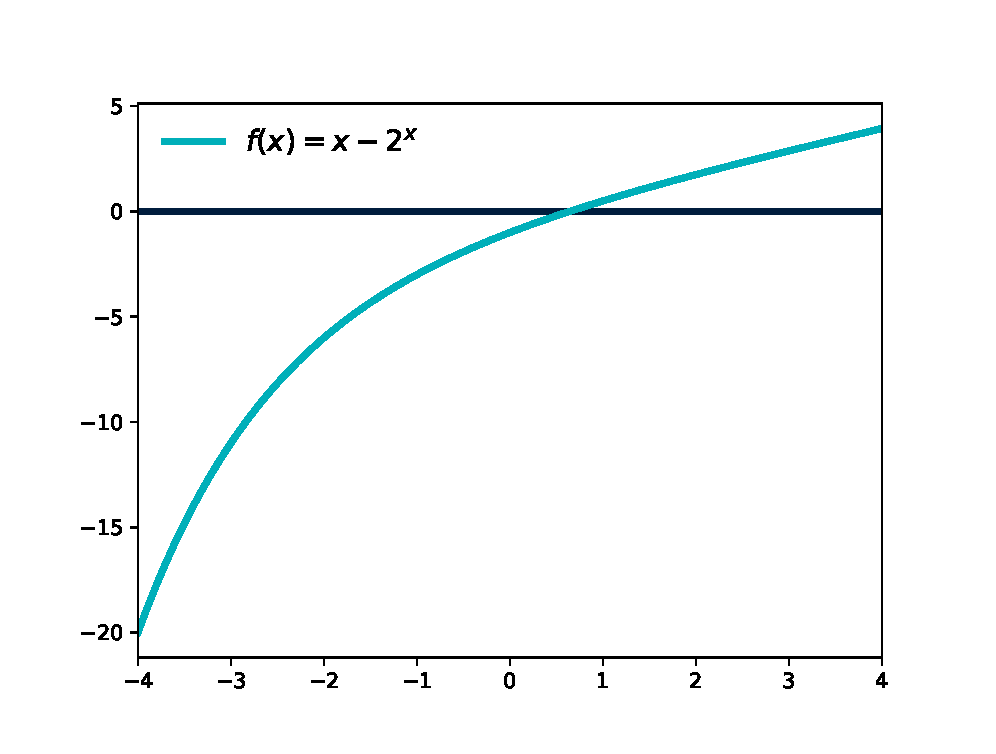
\includegraphics[width=10cm]{Graphics/function_1.eps}
              \caption{Función: $f(x)=x-2^{-x}$ en el intervalo $[-4,4]$.}
              \label{fig:problema1a}
          \end{figure}
          donde se aprecia que su solución se encuentra en el intervalo de $[-1,1]$. Análiticamente podemos comprbar este resultado usando el teorema de Bolzano. Evaluando $f(-1)$ y $f(1)$, obtenemos lo siguiente:
          \begin{align*}
              f(-1) & = -1-2^{-(-1)} & \qquad f(1) & = 1-2^{-1}     \\
                    & =1-2           & \qquad      & =1-\frac{1}{2} \\
                    & =-1            & \qquad      & =\frac{1}{2}
          \end{align*}
          como $f(-1)<0$ y $f(1)>0$, entonces entre $[-1,1]$ se encuentra la solución de la ecuación.
    \item $2xcos(2x)-(x+1)^2=0$\\
          Sea $f(x)=2xcos(2x)-(x+1)^2$, en el caso de esta función, al estar compuesta de una función periodica y un polinomio es complicado obtener puntos importantes como serían los valores críticos y puntos de inflexión. Por lo que se optara por realizar una gráifca de la función. Se eliguio el intervalo de $[-4,4]$, porque $(x+1)^2$ obtiene valores más grandes en comparación a $2xcos(2x)$ en el dominio de la función. Provocando que la función $f(x)$ obtenga valores negativos. Observando la figura \ref{fig:problema1b} se comprueba lo antes dicho, entonces los intervalos que para la solución del problema son $[-2,-0.5]$ y $[0,0.5]$
          \begin{figure}[H]
              \centering
              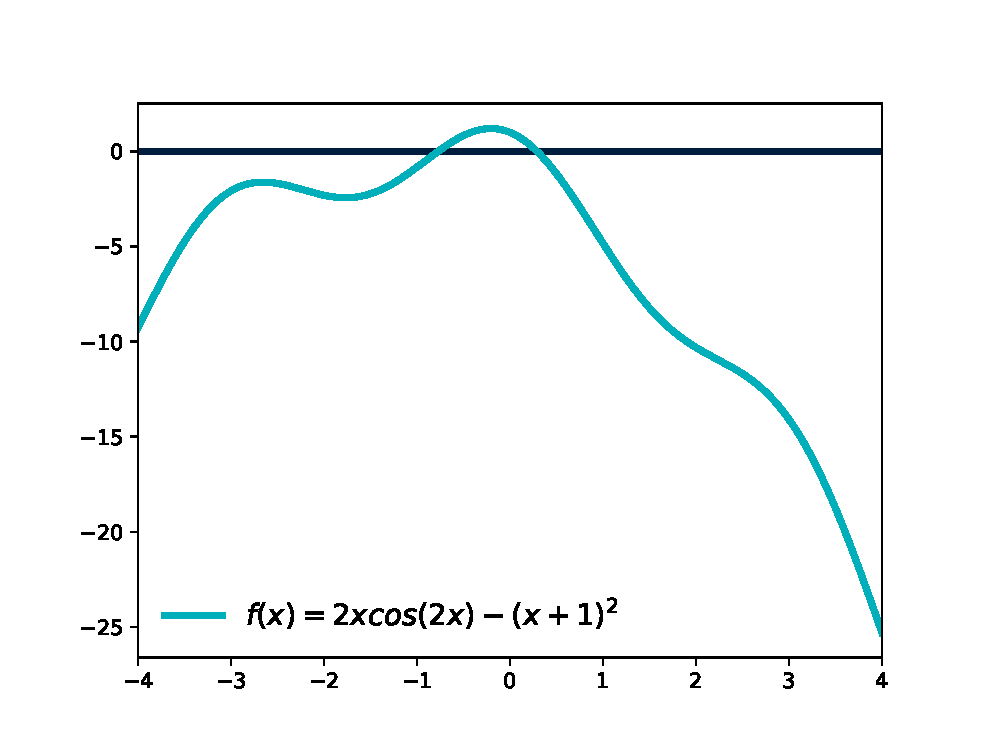
\includegraphics[width=7cm]{Graphics/function_2.eps}
              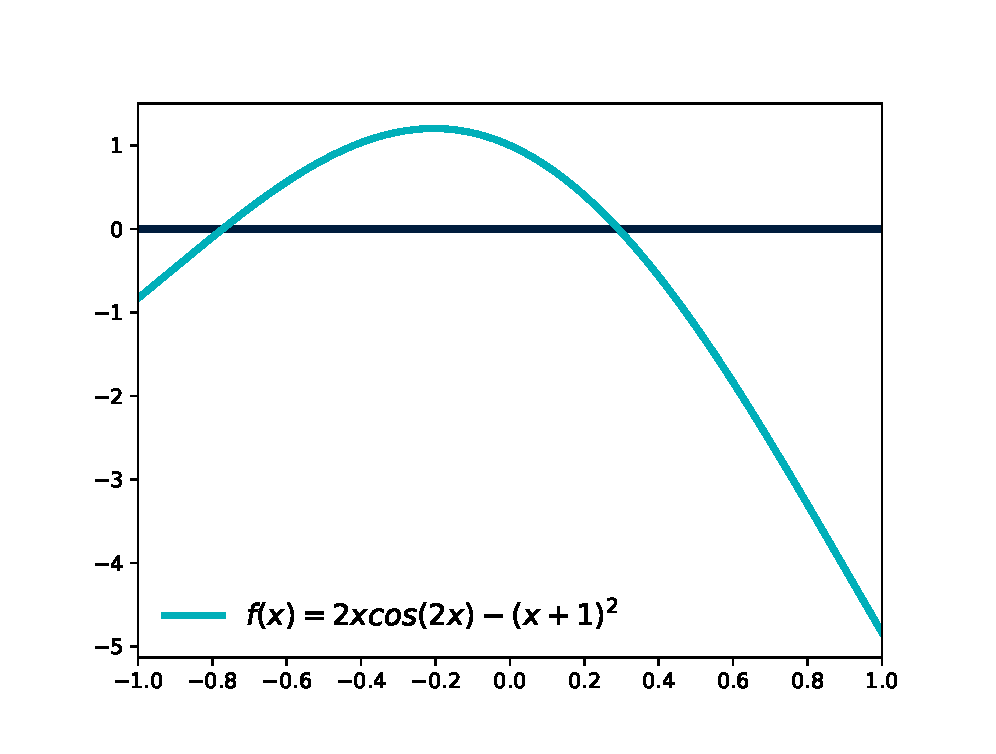
\includegraphics[width=7cm]{Graphics/function_2b.eps}
              \caption{Función: $f(x)=2xcos(2x)-(x+1)^2=0$ en el intervalo $[-4,4]$ (izquierda) y  en el intervalo $[-1,1]$ (derecha).}
              \label{fig:problema1b}
          \end{figure}
          Análiticamente podemos comprbar este resultado usando el teorema de Bolzano. Evaluando $f(-2)$ y $f(-0.5)$ obtenemos lo siguiente:
          \begin{align*}
              f(-2) & =  -2.307 & \qquad f(-0.5) & = 0.831
          \end{align*}
          como $f(-2)<0$ y $f(-0.5)>0$, entonces en el intervalo $[-2,0.831]$ se encuentra una solución de la ecuación.\\
          De igual manera, evaluando $f(0)$ y $f(0.5)$ obtenemos lo siguiente:
          \begin{align*}
              f(0) & =  1 & \qquad f(0.5) & = -1.169
          \end{align*}
          como $f(0.5)<0$ y $f(0)>0$, entonces en el intervalo $[0,0.5]$ se encuentra una solución de la ecuación.
\end{enumerate}